\documentclass[amsmath,amssymb,aps,prd,10pt,twocolumn,showkeys]{revtex4}
\usepackage{graphicx}
\usepackage{mathtools}
\usepackage{empheq}
\usepackage{verbatim}
\DeclareMathOperator\erfc{erfc}
\DeclareMathOperator\erf{erf}
\DeclareMathOperator{\sgn}{sgn}
\begin{document}

\title{Complex Analysis of Askaryan Radiation: Towards UHE-$\nu$ energy Reconstruction via the Hilbert Envelope of Observed Signals}

\author{Jordan C. Hanson}
\email{jhanson2@whittier.edu}
\affiliation{Department of Physics and Astronomy, Whittier College}
\author{Raymond Hartig}
\affiliation{Department of Physics and Astronomy, Whittier College}
\date{\today}

\begin{abstract}
This is a work in progress.
\end{abstract}

\keywords{Ultra-high energy neutrino; Askaryan radiation; Mathematical physics}

\maketitle

\section{Introduction}

The introduction.

\section{Units, Definitions, and Conventions}
\label{sec:unit}

The units.

\section{Collection of Main Results}
\label{sec:onc}

Here is a list of the basic results and ideas for this paper.

\begin{itemize}
\item Let the signal model $s(t)$ be
\begin{equation}
s(t) = -E_0 t e^{-\frac{1}{2}\left(t/\sigma_t\right)^2} \label{eq:s}
\end{equation}
This is the off-cone field equation from \cite{PhysRevD.105.123019}.  The parameter $\sigma_{\rm t}$ is the pulse width, and it depends two quantities: the longitudinal length of the UHE-$\nu$-induced cascade, and the angle at which the cascade is observed relative to the Cherenkov angle.  The parameter $E_0$ is the amplitude normalization, and it depends on two parameters: $\sigma_{\rm t}$, and $\omega_{\rm 0}$, the cutoff frequency from the cascade form factor.
\item Let $\widehat{s}(t)$ represent the Hilbert transform of $s(t)$.  The \textit{analytic signal} of $s(t)$ is
\begin{equation}
s_{\rm a}(t) = s(t) + j \widehat{s}(t)
\end{equation}
The magnitude of the analytic signal, $|s_a(t)|$, is the \textit{envelope} of the signal.  The Hilbert transform $\widehat{s}(t)$ is equivalent to the convolution of $s(t)$ and the tempered distribution $h(t) = 1/(\pi t)$.
\item Let $S(f)$ be the Fourier transform of $s(t)$.  The Fourier transform of the analytic signal is
\begin{equation}
\mathcal{F}\lbrace s_{\rm a}(t) \rbrace_{f} = S_{\rm a}(f) = S(f)(1+\sgn{f}) \label{eq:sa_1}
\end{equation}
The sign function, $\sgn$ gives $-1$ if $f<0$, $0$ if $f=0$, and $1$ if $f>1$.
\item Taking the inverse Fourier transform of Eq. \ref{eq:sa_1}, the analytic signal may be written in terms of $S(f)$:
\begin{equation}
s_{\rm a}(t) = 2\int_{0}^{\infty} S(f) e^{2\pi j f t} df \label{eq:sa_2}
\end{equation}
\item The Fourier transform of Eq. \ref{eq:s} is
\begin{equation}
S(f) = E_0 \sigma_t^3 (2\pi)^{3/2} j f e^{-2\pi^2 f^2 \sigma_t^2}
\end{equation}
\item Using the gaussian spectral width $\sigma_{\rm f}$ from \cite{10.1016/j.astropartphys.2017.03.008}, and the guassian width of $s(t)$ from \cite{PhysRevD.105.123019}, it was shown in \cite{PhysRevD.105.123019} that the uncertainty principle holds for off-cone signals:
\begin{equation}
\sigma_t \sigma_f \geq \frac{1}{2\pi}
\end{equation}
The equality is reached in the limit the far-field parameter limits to zero: $\eta \to 0$.  This makes the signal spectrum
\begin{equation}
S(f) = E_0 \sigma_t^3 (2\pi)^{3/2} j f e^{-\frac{1}{2}\left(f/\sigma_f\right)^2} \label{eq:spec}
\end{equation}
Inserting $S(f)$ into Eq. \ref{eq:sa_2}, $s_{\rm a}(t)$ is
\begin{equation}
s_{\rm a}(t) = \frac{E_0 \sigma_t^3 (2\pi)^{3/2}}{\pi} \frac{d}{dt}\int_0^{\infty} e^{-\frac{1}{2}\left(f/\sigma_f\right)^2} e^{2\pi j f t} df \label{eq:sa_3}
\end{equation}
\item Let $k^2/4 = \frac{1}{2}\left(f/\sigma_f\right)^2$, and $x = t/(\sqrt{2}\sigma_t)$.  Equation \ref{eq:sa_3} can be broken into real and imaginary parts:
\begin{align}
s_{\rm a}(t) &= \frac{E_0 \sigma_{\rm t}}{\sqrt{2\pi}}\frac{dI}{dx} \\
\Re\lbrace I \rbrace &= \int_0^{\infty} e^{-k^2/4}\cos(kx) dk \\
\Im\lbrace I \rbrace &= \int_0^{\infty} e^{-k^2/4}\sin(kx) dk
\end{align}
The real part of $I$ is even, so it can be extended to $(-\infty,\infty)$ if it is multiplied by $1/2$.  The result is
\begin{equation}
\Re\lbrace I \rbrace = \sqrt{\pi} e^{-x^2}
\end{equation}
The imaginary part of $I$ is proportional to \textit{Dawson's integral, $D(x)$:}
\begin{equation}
\Im\lbrace I\rbrace = 2 D(x)
\end{equation}
\item The overall analytic signal, $s_a(t)$, is
\begin{equation}
s_a(t) = -E_0 \left(t e^{-\frac{1}{2}\left(t/\sigma_t\right)^2} - \frac{2 j\sigma_t}{\sqrt{2\pi}} \frac{dD(x)}{dx}\right) \label{eq:sa_4}
\end{equation}
The signal envelope is $|s_a(t)|$.  It is important to note that, though $D(x)$ is not evaluated analytically, a high-precision algorithm for computing $D(x)$ was given in \cite{10.1063/1.4822832}.  Note that $s_a(0) \neq 0$, since $dD(x)/dx = 1 - 2x D(x)$.
\item Signal data in detectors designed to observe Askaryan pulses is equivalent to the convolution of the signal and detector response functions.  Signal models are convolved with measured detector responses to create \textit{signal templates}.  Signal templates are cross-correlated with observed data to identify UHE-$\nu$ signals.  The oscillations of signal templates and observed data can introduce various uncertainties when cross-correlated.  This problem intensifies when the signal-to-noise ratio between Askaryan pulse data and thermal noise decreases.  To reduce these uncertainties, the Hilbert envelope of observed signals is used in cross-correlations instead of the original signals.  We seek an analytic equation for the Hilbert envelope of the data.  That is, we seek the envelope of the convolution of the analytic signal model with a typical detector response.  The RLC damped oscillator is a standard circuit model for the RF dipole antennas used in RNO-G and the proposed IceCube Gen2 \cite{10.1103/PhysRevD.85.062004,10.1088/1748-0221/16/03/p03025,10.48550/arxiv.2008.04323}.
\item There are two paths to calculating the final result.  The first option involves three steps.  First, the detector response, $r(t)$ is convolved with $s(t)$.  Second, the analytic signal of the result is found.  Third, the magnitude of the analytic signal is computed, which can be compared to envelopes of observed signals.  The second option involves computing the envelope of the convolution of $r(t)$ with $s(t)$ directly from $s_a(t)$ and $r_a(t)$.
\item Let $s(t) * r(t)$ represent the convolution of $s(t)$ and $r(t)$.  Let the envelope of the convolution be $\mathcal{E}_{s * r}(t)$.  $\mathcal{E}_{s * r}(t)$, $s_a(t)$, and $r_a(t)$ are related by
\begin{equation}
\mathcal{E}_{s * r}(t) = \frac{1}{2}| s_a (t) * r_a(t)| \label{eq:awesome}
\end{equation}
The proof of Eq. \ref{eq:awesome} is based on two ideas.  First, the Hilbert transform of a function $s(t)$ is equivalent to convolving it with the ``tempered distribution'' $h(t) = 1/(\pi t)$.  Second, computing the Hilbert transform twice yields the original function, multiplied by $-1$: $h * h * s = -s$.  Given the definitions of the analytic signal and the Hilbert transform,
\begin{align}
(s * r)_a (t) &= s * r + j ~ \widehat{s*r} \\
\mathcal{E}_{s * r}(t) &= | s * r + j s * r * h|
\end{align}
However,
\begin{align}
r_a * s_a &= (r + j \hat{r}) * (s + j \hat{s}) \\
r_a * s_a &= r * s + j r * \hat{s} + j \hat{r} * s - \hat{r} * \hat{s} \\
r_a * s_a &= r * s - r * h * s * h + 2 j h * r * s \\
r_a * s_a &= r * s - h * h * r * s + 2 j h * r * s \\
r_a * s_a &= 2 r * s + 2 j h * r * s
\end{align}
Multiplying both sides $1/2$ and taking the magnitude completes the proof:
\begin{equation}
\frac{1}{2} |r_a * s_a| = |r * s + j h * r * s| = \mathcal{E}_{s * r}(t) \\
\end{equation}
\item The RLC damped oscillator impulse response and corresponding analytic signal are
\begin{align}
r(t) &= R_0 e^{-2 \pi \gamma_f t} \cos(2\pi f_0 t) \label{eq:r} \\
r_a(t) &= R_0 e^{-2 \pi \gamma_f t} e^{2\pi j f_0 t} \label{eq:ra}
\end{align}
The parameters $\gamma_f$ and $f_0$ are the \textit{decay constant} that corresponds to the \textit{fall time} of the output signal, and the resonance frequency.  Note that the envelope of $r(t)$, $|r_a(t)|$, is $R_0 \exp(-2 \pi \gamma_f t)$, as expected.  To prove Eq. \ref{eq:ra}, first compute the Fourier transform of $r(t)$:
\begin{align}
R(f) &= \frac{R_0}{4\pi j} \left( \frac{1}{f - z_{+}} + \frac{1}{1- z_{-}} \right) \\
z_{+} &= f_0 + j \gamma_f \\
z_{-} &= -f_0 + j \gamma_f
\end{align}
Given Eq. \ref{eq:sa_2}, the procedure to find $r_a(t)$ is to multiply the \textit{negative} frequency components by 0 and the \textit{positive} frequency components by 2, and take the inverse Fourier transform.  The inverse Fourier transform may be completed by extension to the complex plane using the upper infinite semi-circle as a contour, and applying Jordan's lemma.  The residue from the pole at $z_{+}$ drives the final result.
%\item The behavior of the RLC oscillator can be extended to the charging state, and the decaying state, via the time-reversal of Eq. \ref{eq:r}.  Times with $t\leq 0$ correspond to the charging state, $t=0$ corresponds to peak response, and $t\geq 0$ corresponds to the decaying state.  For the charging state:
%\begin{align}
%r(t) &= R_0 e^{2 \pi \gamma_r t} \cos(2\pi f_0 t) \label{eq:rc} \\
%r_a(t) &= R_0 e^{2 \pi \gamma_r t} e^{2\pi j f_0 t} \label{eq:rac}
%\end{align}
%The resonance frequency remains the same as the decaying state, and $\gamma_r$ corresponds to the \textit{rise time} in the same way that $\gamma_f$ corresponds to the \textit{fall time.}  In general, the rise and fall times do not have to be equal.
\item The goal is now to apply Eq. \ref{eq:awesome} by convolving $s_a(t)$ with $r_a(t)$.  The real part of $s_a(t)$ can be convolved with $r_a(t)$ in the time domain.  As in Eq. \ref{eq:sa_4}, real part of $s_a(t)$ is $s(t)$.  Since $r_a(t<0)=0$, the convolution is written
\begin{equation}
r_a(t) * \Re\lbrace s_a(t) \rbrace = \int_0^{\infty} r_a(\tau) s(t-\tau) d\tau
\end{equation}
Let $x=t/(\sqrt{2}\sigma_t)$, $y=\tau/(\sqrt{2}\sigma_t)$, and $z_0 = \sqrt{2}\sigma_t(\gamma-2\pi jf_0)$. The convolution may be organized as follows
\begin{equation}
r_a(t) * \Re\lbrace s_a(t) \rbrace = R_0 s(t) I + R_0 E_0 \sigma_t^2 e^{-\frac{1}{2}(t/\sigma_t^2)} \frac{dI}{dt} \label{eq:conv}
\end{equation}
with
\begin{equation}
I(x,z_0) = \sqrt{2}\sigma_t \int_0^{\infty} e^{-y^2 + (2x-z_0)y} dy
\end{equation}
Let $b = x-z_0/2$. Completing the square in the exponent produces
\begin{equation}
I(x,z_0) = \sqrt{2}\sigma_t e^{b^2} \int_0^{\infty} e^{-(y-b)^2} dy
\end{equation}
The integral may be cast as a complementary error function by substituting $u=y-b$ and letting $b=jz$:
\begin{equation}
I(x,z_0) = \sqrt{\frac{\pi}{2}}\sigma_t e^{-z^2}\erfc(-jz)
\end{equation}
Thus, the integral is proportional to the \textit{Faddeeva function}, $w(z)$:
\begin{equation}
I(x,z_0) = \sqrt{\frac{\pi}{2}} \sigma_t w(z) \label{eq:fadd}
\end{equation}
Substituting Eq. \ref{eq:fadd} into Eq. \ref{eq:conv}, and simplifying, produces
\begin{multline}
r_a(t) * \Re\lbrace s_a(t) \rbrace = \sqrt{\frac{\pi}{2}}R_0 \sigma_t s(t) w(z) \\
-j\frac{\sqrt{\pi}}{2} R_0 E_0 \sigma_t^2 e^{-\frac{1}{2}(t/\sigma_t)^2} \frac{dw(z)}{dz} \label{eq:Re_result}
\end{multline}
\item Turning to the convolution of $r_a(t)$ with $\Im(s_a)$, note that the imaginary part of Eq. \ref{eq:sa_4} contains $dD(x)/dx$, the derivative of the Dawson function.  To complete the convolution, the inverse Fourier transform of the product of the Fourier transforms of $r_a(t)$ and $\Im\lbrace s_a(t)\rbrace$ is calculated.  To complete this step, the Fourier transform of $dD(x)/dx$ is needed:
\begin{align}
x &= t/(\sqrt{2}\sigma_t) \\
f' &= \sqrt{2} \sigma_t f \\
\mathcal{F}\left\lbrace \frac{dD(x)}{dx}\right\rbrace &= \int_{-\infty}^{\infty} \frac{dD(x)}{dx}e^{-2\pi jft} dt \\
\mathcal{F}\left\lbrace \frac{dD(x)}{dx}\right\rbrace &= \sqrt{2}\sigma_t(2\pi jf') \int_{-\infty}^{\infty} D(x) e^{-2\pi jf'x} dx \\
\mathcal{F}\left\lbrace \frac{dD(x)}{dx}\right\rbrace &= 2\pi^2 \sigma_t^2 f e^{-\frac{1}{2}(f/\sigma_f)^2} \sgn(f)
\end{align}
Let $z_0 = (\gamma - 2\pi jf_0)$, so that the Fourier transform of $r_a$ is 
\begin{align}
\mathcal{F}\left\lbrace r_a(t)\right\rbrace &= R_0\int_{0}^{\infty} e^{-z_0 t} e^{-2\pi j ft} dt \\
\mathcal{F}\left\lbrace r_a(t)\right\rbrace &= \frac{R_0}{z_0+2\pi j f}
\end{align}
Let $z_1 = f_0 + j\gamma/(2\pi)$. Multiplying the Fourier transforms, and simplifying, yields
\begin{multline}
\mathcal{F}\left\lbrace r_a(t) * \Im\left\lbrace s_a(t)\right\rbrace \right\rbrace = \\ -j \sqrt{2\pi} R_0 E_0 \sigma^3 \frac{f\sgn(f) e^{-\frac{1}{2}(f/\sigma_f)^2}}{f-z_1}
\end{multline}
The inverse Fourier transform now gives $r_a(t) * \Im\left\lbrace s_a(t) \right\rbrace$:
\begin{multline}
r_a(t) * \Im\left\lbrace s_a(t) \right\rbrace = \\
-j\sqrt{2\pi} R_0 E_0 \sigma_t^3 \int_{-\infty}^{\infty} \frac{f\sgn(f)e^{-\frac{1}{2}(f/\sigma_f)^2}e^{2\pi jft}}{f-z_1} df
\end{multline}
Let $y = f/(\sqrt{2}\sigma_f)$, $x=t/(\sqrt{2}\sigma_t)$, $\sgn(f) = \sgn(y)$, and $z_1 \to f_0/(\sqrt{2}\sigma_f) + j\gamma/(2\pi \sqrt{2} \sigma_f)$.  The inverse Fourier transform can be organized as:
\begin{multline}
r_a(t) * \Im\left\lbrace s_a(t) \right\rbrace = \\
-\frac{R_0E_0\sigma_t^3}{\sqrt{2\pi}}\frac{d}{dt}\int_{-\infty}^{\infty} \frac{\sgn(y) e^{-y^2+2jxy}}{y-z_1} dy
\end{multline}
Completing the square in the exponent, factoring a unit of $j$ from the exponent, and changing the derivative from $d/dt$ to $d/dx$ gives
\begin{multline}
r_a(t) * \Im\left\lbrace s_a(t) \right\rbrace = \\
-\frac{R_0E_0\sigma_t^2}{2\sqrt{\pi}}\frac{d}{dx}e^{-x^2} \int_{-\infty}^{\infty} \frac{\sgn(y) e^{(x+jy)^2}}{y-z_1}dy
\end{multline}
Let $z = x+jy$, with $y = \Im(z)$.  In this substitution, $x$ is treated as a constant, so $dz = jy$.  Let $z_2 = x+j z_1$, while $z_1 = f_0/(\sqrt{2}\sigma_f) + j\gamma/(2\pi \sqrt{2} \sigma_f)$.  The result is
\begin{multline}
r_a(t) * \Im\left\lbrace s_a(t) \right\rbrace = \\
-\frac{R_0E_0\sigma_t^2}{2\sqrt{\pi}}\frac{d}{dx}e^{-x^2} \int_{x-j\infty}^{x+j\infty} \frac{\sgn(\Im(z)) e^{z^2}}{y-z_2}dz \label{eq:cont_int}
\end{multline}
The integral may be finished by extending $z$ to the complex plane and using contour integration.  The location of the pole is in the first quadrant, unless $t = (\gamma \sigma_t)\sigma_t$.  In that case, $\Re(z_2)=0$, and the pole is located on the imaginary axis.  For typical values of $\sigma_t$ and $\gamma$, $t\approx 0.1$ ns. Since $r(t)=0$ if $t<0$, the location of $z_2$ is usually in the first quadrant.  Let the line integrals of the rectangular contour be: $I_1$, $(x,-jR) \to (x,jR)$, $I_2$, $(x,jR) \to (0,jR)$, $I_3$, $(0,jR) \to (0,-jR)$, and $I_4$, $(0,-jR) \to (x,-jR)$.  $I_2$ and $I_4$ are both proportional to $\exp(-R^2)$, so $I_2 \to 0$ and $I_4 \to 0$ when $R \to \infty$.  $I_1$ is the integral in Eq. \ref{eq:cont_int}.  Let $w = -y$, so that $I_3$ is
\begin{equation}
I_3 = -\int_0^{R} \frac{e^{-y^2}}{y-z_1} dy + \int_0^{R} \frac{e^{-w^2}}{w+z_1} dw
\end{equation}
Integrals of the type in $I_3$ are known as \textit{Goodwin-Staton} functions, and are related to the other error functions.  The Goodwin-Staton function, $G(z_1)$, is odd, so $-G(-z_1) = G(z_1)$.  The result for $I_3$ is
\begin{equation}
I_3 = -G(-z_1) + G(z_1) = 2G(z_1)
\end{equation}
The residue of the enclosed contour $I_C = I_1+I_2+I_3+I_4$ is $\exp(z_2^2)$.  With $I_2$, $I_3$, and $I_4$ completed, the solution for $I_1$ is
\begin{equation}
I_1 = 2\pi j e^{z_2^2} - 2G(z_1)
\end{equation}
Inserting this result into Eq. \ref{eq:cont_int}, and simplifying, gives
\begin{multline}
r_a(t) * \Im\left\lbrace s_a(t) \right\rbrace = \\
-\frac{R_0E_0\sigma_t^2}{2\sqrt{\pi}}\frac{d}{dx}\left( 2\pi j e^{2 j x z_1 - z_1^2} - 2G(z_1) e^{-x^2} \right)
\end{multline}
Notice that $2\pi j x z_1 = 2\pi j f_0 t - \gamma t$.  Evaluating the derivative and simplifying gives the final result:
\begin{multline}
r_a(t) * \Im\left\lbrace s_a(t) \right\rbrace = \\
\sqrt{\pi}E_0 \sigma_t^2 z_1 e^{-z_1^2}r_a(t) + \sqrt{\frac{2}{\pi}} G(z_1) R_0 \sigma_t s(t) \label{eq:Im_result}
\end{multline}
\item Combining Eq. \ref{eq:Re_result} and Eq. \ref{eq:Im_result} gives $r_a(t) * s_a(t)$:
\begin{multline}
r_a(t) * s_a(t) = \\
\sqrt{\frac{\pi}{2}}R_0 \sigma_t s(t) w(z) - j\frac{\sqrt{\pi}}{2} R_0 E_0 \sigma_t^2 e^{-\frac{1}{2}(t/\sigma_t)^2} \frac{dw(z)}{dz} + \\
j\sqrt{\pi}E_0 \sigma_t^2 z_1 e^{-z_1^2}r_a(t) + j\sqrt{\frac{2}{\pi}} G(z_1) R_0 \sigma_t s(t) \label{eq:final}
\end{multline}
The units of convolution should be $R_0 E_0\sigma_t^2$, and each term in Eq. \ref{eq:final} has these units.  The first term is proportional to $R_0 \sigma_t s(t)$, and $s(t)$ has units of $E_0 \sigma_t$, so the unit product is $R_0 E_0\sigma_t^2$.  The units of the second term are $R_0 E_0\sigma_t^2$.  The third term has units of $E_0\sigma_t^2 r_a(t)$, and $r_a(t)$ has units of $R_0$, so the unit product is $R_0 E_0\sigma_t^2$.  The fourth term has units of $R_0 \sigma_t s(t)$, like the first term.  Thus, all units check.  To check the limits, the parameters within $z$ and $z_1$ must be recalled.  Combining prior definitions, the results are
\begin{align}
z &= \sqrt{2}\sigma_t \pi f_0 + j\left(\frac{\sigma_t\gamma}{\sqrt{2}} - x\right) \\
z_1 &= f_0/(\sqrt{2}\sigma_f) + j\gamma/(2\pi \sqrt{2} \sigma_f)
\end{align}
Recall that $\sigma_t = 1/(2\pi \sigma_f)$, and $x=t/(\sqrt{2}\sigma_t)$.  Substituting this into the definition of $z$ reveals that
\begin{equation}
z_1 = z + jx
\end{equation}
Thus, when $t=0$, the two poles are equal, since $t=0$ means $x=0$.  Taking the magnitude of Eq. \ref{eq:final}, and multiplying by $1/2$, gives the final result:
\begin{equation}
\mathcal{E}_{r * s}(t) = \frac{1}{2} | r_a(t) * s_a(t) |
\end{equation}
\item Two examples of comparisons of Eq. \ref{eq:final} to the convolution of $s(t)$ and $r(t)$ are given in Fig. \ref{fig:fig1} below.
\begin{figure}[hb]
\centering
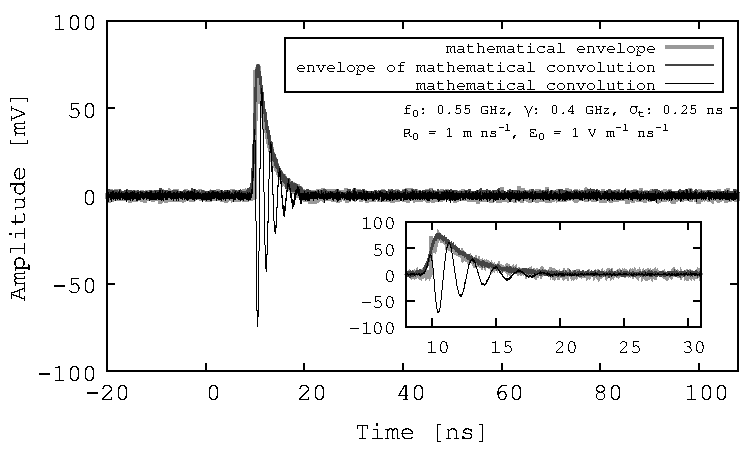
\includegraphics[width=0.5\textwidth]{March12_plot1.pdf}
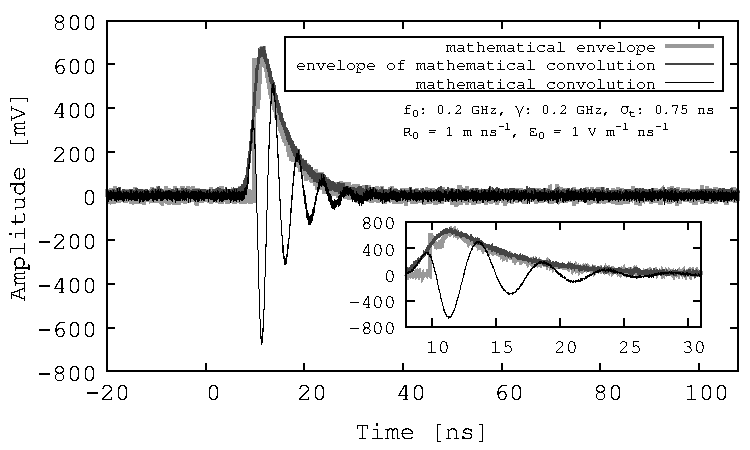
\includegraphics[width=0.5\textwidth]{March12_plot2.pdf}
\caption{\label{fig:fig1} (Top) The thin black line represents $s(t) * r(t)$.  The dark gray envelope represents the envelope of $s(t) * r(t)$ computed with the Python3 package scipy.special.hilbert. The light gray envelope represents Eq. \ref{eq:final}. (Bottom) Same as top, for different parameter values.}
\end{figure}
\item It is important to note that the convolution of $s(t)$ and $r(t)$ may be done analytically in the time-domain.  Starting with the definitions of $s(t)$, $r(t)$, and the convolution integral:
\begin{align}
s * r &= \int_0^{\infty} r(\tau) s(t-\tau) d\tau \\
s * r &= -E_0 \int_0^{\infty} r(\tau) (t-\tau) e^{-\frac{1}{2}\left(\frac{t-\tau}{\sigma_t}\right)^2}d\tau \\
s * r &= \left(s(t) + E_0 \sigma_t^2 e^{-\frac{1}{2}\left(\frac{t}{\sigma_t}\right)^2} \frac{d}{dt} \right)I(t,\sigma_t) \label{eq:conv_1} \\
I(t,\sigma_t) &= \int_0^{\infty} r(\tau) e^{(t\tau)/\sigma_t^2} e^{-\frac{1}{2}\left(\frac{\tau}{\sigma_t}\right)^2}d\tau
\end{align}
To compute $I(t,\sigma_t)$, let
\begin{align}
z &= \gamma - 2\pi j f_0 \\
z_0 &= \sqrt{2}\sigma_t z\\
x &= t/(\sqrt{2} \sigma_t) \\
y &= \tau/(\sqrt{2} \sigma_t) \\
r(\tau) &= \Re\left\lbrace R_0 e^{-z\tau}\right\rbrace
\end{align}
These substitutions simply $I(t,\sigma_t)$ to
\begin{equation}
I(t,\sigma_t) = \sqrt{2} \sigma_t R_0 \Re \left\lbrace\int_0^{\infty} e^{(2y-z_0)x} e^{-x^2} dx \right\rbrace
\end{equation}
Let $b = y-z_0/2$, Completing the square in the exponent gives
\begin{equation}
I(t,\sigma_t) = \sqrt{\frac{\pi}{2}} \sigma_t R_0 \Re\left\lbrace e^{b^2} \erfc(-b) \right\rbrace
\end{equation}
Let $b = jc$, so that
\begin{align}
I(t,\sigma_t) &= \sqrt{\frac{\pi}{2}} \sigma_t R_0 \Re\lbrace e^{-c^2} \erfc(-jc) \rbrace \\
I(t,\sigma_t) &= \sqrt{\frac{\pi}{2}} \sigma_t R_0 \Re\lbrace w(c) \rbrace
\end{align}
The Faddeeva function $w(z)$ may be broken into real and imaginary parts using the Voigt functions:
\begin{equation}
U(p,q) + jV(p,q) = \sqrt{\frac{\pi}{4q}} w(z)
\end{equation}
The relationship between $p$, $q$, and $z$ is $z=(1-jp)/(2\sqrt{q})$.  Using this relationship, we find
\begin{align}
p &= \left(\frac{t}{\sigma_t}\right)\left(\frac{\sigma_f}{f_0}\right) - \frac{\gamma}{2\pi f_0} \\
q &= \frac{1}{2}\left(\frac{\sigma_f}{f_0}\right)^2
\end{align}
Thus, the integral $I(t,\sigma_t)$ becomes
\begin{equation}
I(t,\sigma_t) = \sigma_t R_0 \left(\frac{\sigma_f}{f_0}\right) U(p,q)
\end{equation}
Substituting the result for $I(t,\sigma_t)$ in Eq. \ref{eq:conv_1} gives
\begin{multline}
s * r = \\
 R_0\sigma_t \left(\frac{\sigma_f}{f_0}\right) \left(s(t) + E_0 \sigma_t^2 e^{-\frac{1}{2}\left(\frac{t}{\sigma_t}\right)^2} \frac{d}{dt} \right) U(p,q) \label{eq:conv_2}
\end{multline}
Equation \ref{eq:conv_2} can be simplified in two ways.  First, note that $\sigma_t \sigma_f = 1/(2\pi)$, so $R_0\sigma_t (\sigma_f/f_0) = R_0/(2\pi f_0)$.  Second, the derivative of the Voigt function may be simplified using the chain rule:
\begin{equation}
\frac{dU(p,q)}{dt} = \frac{dU(p,q)}{dp}\frac{dp}{dt} = \frac{dU(p,q)}{dp} \frac{\sigma_f}{\sigma_t f_0}
\end{equation}
Thus, Eq. \ref{eq:conv_2} becomes
\begin{multline}
s * r = \\
\frac{R_0}{2\pi f_0}\left(s(t) + E_0 \sigma_t \left(\frac{\sigma_f}{f_0}\right) e^{-\frac{1}{2}\left(\frac{t}{\sigma_t}\right)^2} \frac{d}{dp}\right)U(p,q) \label{eq:conv_3}
\end{multline}
The envelope of Eq. \ref{eq:conv_3} can be computed numerically, which represents an alternative approach to that represented by Eq. \ref{eq:awesome}.
\end{itemize}

\section{Conclusion}
\label{sec:conc}

The conclusion.

\appendix

\section{Details}
\label{app:a}

The details.

\bibliography{apssamp}

\end{document}

